% This was one of the better templates that I used for the tex.stackexchange.com
% competition. Based on minipages and a bit of pulling and pushing. If you want to
% get fussy, some improvements in kerning are necessary. The left
% bottom caption was pushed using a rule. Set the rule height to 1pt to see
% how it was done.
% Dr Y Lazarides 2012
% 
\documentclass[imperial]{octavo}
\usepackage[top=1cm,right=1cm,left=1cm]{geometry}
\usepackage{graphicx}
\usepackage{caption}
\usepackage{multicol}
\usepackage{ragged2e}
\long\def\note{%
   \begin{minipage}[b]{2cm}
   \RaggedRight
   University of Pensylvania medical students for \$750. But Thomas Eskins became
                                   so interested that he painted an entire cancer operation,
                                    with portraits of student spectators thrown in.
  \end{minipage}
}
\parindent0pt
\begin{document}
%%%%%%%%%%%% DR AGNEW PAGE
\fboxrule0.3pt
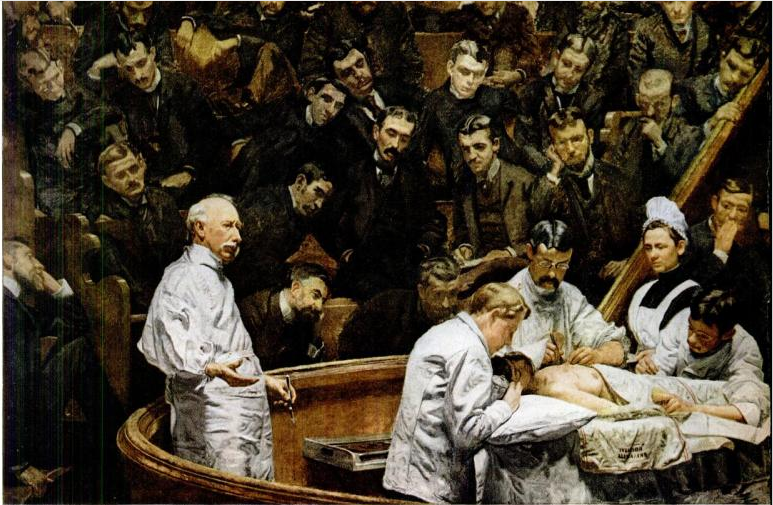
\includegraphics[width=1.0\textwidth]{agnewesclinic}\par
\vspace{-\baselineskip}
\begin{multicols}{3}
\noindent \footnotesize\textbf{``The Agnew Clinic''} started out as a portrait of the famous surgeon Dr. D. Hayes Agnew,  who is shown with scalpel in his hand at left. The picture was commissioned by
University of Pensylvania medical students for \$750. But Thomas Eskins became so interested that he painted an entire cancer operation, with portraits of student spectators thrown in.
\end{multicols}

\rule{1.9cm}{0pt}\llap{\note}\fbox{%
\begin{minipage}[t]{0.9\textwidth}
\begin{minipage}[t]{0.45\textwidth}
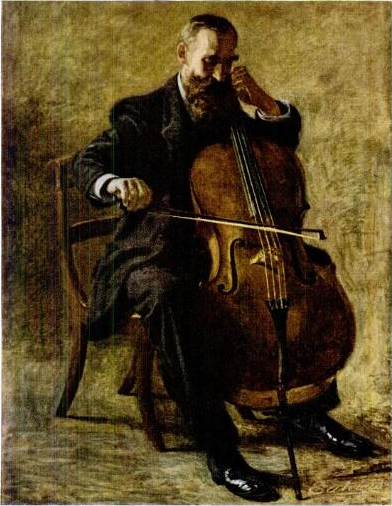
\includegraphics[width=1\textwidth]{celloplayer}\par\vspace*{-8pt}%
\captionof*{figure}{\noindent\footnotesize\textbf{The Cello Player}, is Rudolf Hesting a famous musician in the 1870s. In 1907 a year after
he painted it, Thomas Easkins sold the canvas for \$500, he then gave \$250 to Hesting for posing.}
\end{minipage}\hspace{1.5\columnsep}
\begin{minipage}[t]{0.45\textwidth}
   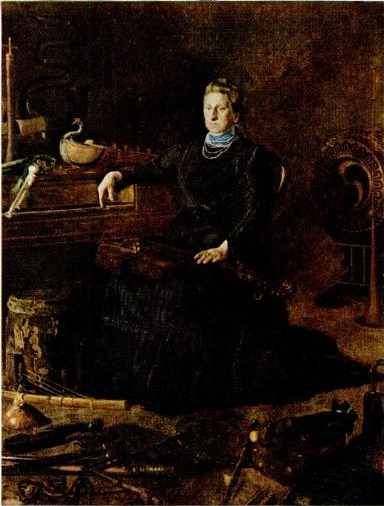
\includegraphics[width=1\textwidth]{mrswilliam}\vspace*{-8pt}
    \captionof*{figure}{\noindent\footnotesize\textbf{Mrs William Frischmoth},
of Philadelphia sat for her portrait in 1900 amid a serpent, an oriental oboy, a burdy-gurdy and other strange musical instruments which she collected.}
\end{minipage}
\end{minipage}
}
\end{document}